\documentclass{article}
\usepackage{hyperref}
\usepackage{Style}

\nocite{*} % Comentar si quiero citar
%\addbibresource{bibliografia.bib} % Quitar el comentado si quiero usar bibliografia

\begin{document}

\begin{minipage}{2.5cm}
    \includegraphics[width=2cm]{imagen_puc.jpg}
\end{minipage}
\begin{minipage}{14cm}
    {\sc Pontificia Universidad Católica de Chile\\
    Facultad de Matemáticas\\
    Departamento de Matemática\\
    Profesora: Amal Taarabt -- Estudiante: Benjamín Mateluna}
\end{minipage}
\vspace{1ex}

{\centerline{\bf Teoría Espectral - MAT2820}
\centerline{\bf Tarea 1}}
\centerline{\bf 15 de septiembre de 2025}

\section{Transformada de Fourier - Versión continua}
\subsection{Propiedades básicas}
\begin{enumerate}
    \item Veamos que para todo $\xi\in\R$ se tiene que $\abs{\F(f)(\xi)}<\infty$, en efecto,
    \begin{equation*}
        \abs{\int_{\R}e^{-ix\xi}f(x)\hspace{1mm}dx}\leq\int_{\R}\abs{e^{-ix\xi}f(x)}\hspace{1mm}dx
        =\int_{\R}\abs{f(x)}\hspace{1mm}dx<\infty
    \end{equation*}
    donde la última desigualdad se obtiene de que $f\in L^{1}(\R)$. Lo anterior implica que 
    $\hat{f}(\xi)\in\C$.

    \item En primer lugar, se tiene que
    \begin{align*}
        \F(g_{1})(\xi) &= \frac{1}{\sqrt{2\pi}}\int_{\R}e^{-ix\xi}e^{-\abs{x}}\hspace{1mm}dx
        =\frac{1}{\sqrt{2\pi}}\int_{\R}e^{-ix\xi-\abs{x}}\hspace{1mm}dx
        =\frac{1}{\sqrt{2\pi}}\left(\int_{\R_{\geq0}}e^{-x-ix\xi}\hspace{1mm}dx
        +\int_{\R_{\leq0}}e^{x-ix\xi}\hspace{1mm}dx\right) \\[2mm]
        &= \frac{1}{\sqrt{2\pi}}\left(-\frac{e^{-x(1+i\xi)}}{1+i\xi}\Big|_{0}^{\infty}
        +\frac{e^{x(1-i\xi)}}{1-i\xi}\Big|_{-\infty}^{0}\right)
        =\frac{1}{\sqrt{2\pi}}\cdot\frac{2}{1+\xi^{2}}
    \end{align*}

    \vspace{2mm}
    Por otro lado, para $g_{2}$, definimos la función compleja $f:\C\to\C$ dada por
    \begin{equation*}
        f(z)=\frac{e^{-iz\xi}}{1+z^{2}}
    \end{equation*}
    Consiramos el siguiente camino en $\C$,
    \begin{center}
        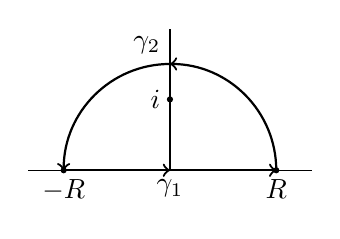
\begin{tikzpicture}[scale=0.9] %Dominio de integración
            \draw[thick, ->] (1.5,0) arc (0:90:1.5);
            \draw[thick, ->] (0,1.5) arc (90:180:1.5);
            
            \coordinate (O) at (0,0);
            \coordinate (A) at (2,0);
            \coordinate (B) at (-2,0);
            \coordinate (C) at (0,2);

            \draw (A) -- (B);
            \draw (O) -- (C);

            \draw[thick, ->] (-1.5,0) -- (0,0);
            \draw[thick, ->] (0,0) -- (1.5,0);

            \filldraw (0,1.5) node[anchor=south east]{$\gamma_{2}$};
            \filldraw (0,0) node[anchor=north]{$\gamma_{1}$};
            \filldraw (-1.5,0) circle (1pt) node[anchor=north]{$-R$};
            \filldraw (1.5,0) circle (1pt) node[anchor=north]{$R$};

            \filldraw (0,1) circle (1pt) node[anchor=east]{$i$};
        \end{tikzpicture}
    \end{center}
    donde $\gamma_{1}(t)=t$ con $t\in[-R,R]$ y $\gamma_{2}(t)=Re^{\pi it}$ para $t\in[0,1]$. 
    Diremos que $\gamma=\gamma_{1}+\gamma_{2}$. Para $R>1$ suficientemente grande se tiene que 
    $i$ esta en la región determinada por $\gamma$, así, por teorema del residuo, se sigue que
    \begin{equation*}
        2\pi i\cdot Res(f,i)=\int_{\gamma}f(z)\hspace{1mm}dz=\int_{\gamma_{1}}f(z)\hspace{1mm}dz
        +\int_{\gamma_{2}}f(z)\hspace{1mm}dz=\int_{-R}^{R}\frac{e^{-it\xi}}{1+t^{2}}\hspace{1mm}dt
        +\int_{0}^{1}\frac{e^{-iRe^{i\pi t}\xi}}{1+R^{2}e^{2\pi it}}\cdot Ri\pi e^{i\pi t}
        \hspace{1mm}dt
    \end{equation*}
    como $i$ es un polo simple de $f$, vemos que
    \begin{equation*}
        Res(f,i)=\lim\limits_{z\to i}(z-i)f(z)=\lim\limits_{z\to i}\frac{e^{-iz\xi}}{z+i}
        =-\frac{i}{2}e^{\xi}
    \end{equation*}
    Por otro lado, tenemos que
    \begin{align*}
        \abs{\int_{0}^{1}\frac{e^{-iRe^{i\pi t}\xi}}{1+R^{2}e^{2\pi it}}\cdot Ri\pi e^{i\pi t}
        \hspace{1mm}dt}\leq\int_{0}^{1}\frac{R\pi e^{Rsen(\pi t)\xi}}{\abs{1+R^{2}e^{2\pi it}}}
        \hspace{1mm}dt\leq\int_{0}^{1}\frac{R\pi e^{Rsen(\pi t)\xi}}{R^{2}-1}\hspace{1mm}dt
    \end{align*}
    
    \item Consideremos la función
    \begin{equation*}
        G(x,\xi)=e^{-ix\xi}\cdot e^{-\frac{x^{2}}{2}}=e^{-(ix\xi+\frac{x^{2}}{2})}
    \end{equation*}
    notemos que $g_{\xi_{0}}(x)=G(x,\xi_{0})$ es continua, por ende es medible, también se tiene 
    que $\pdv{G}{\xi}$ existe para todo $(x,\xi)\in\R^{2}$ y además $g_{0}(x)$ es integrable.
    Veamos que
    \begin{equation*}
        \abs{\pdv{G}{\xi}(x,\xi)}\leq e^{-\frac{x^{2}}{2}}\in L^{1}(\R)
    \end{equation*}
    Así, derivando bajo el signo de la integral se obtiene que
    \begin{align*}
        (\F(f))'(\xi) &= \frac{-i}{\sqrt{2\pi}}\int_{\R}xe^{-\frac{x^{2}}{2}}
        e^{-ix\xi}\hspace{1mm}dx=\frac{-i}{\sqrt{2\pi}}\left(-e^{-\frac{x^{2}}{2}}e^{-ix\xi}
        \Big|_{-\infty}^{\infty}-i\xi\int_{\R}e^{-\frac{x^{2}}{2}}e^{-ix\xi}\hspace{1mm}dx
        \right) \\[2mm]
        &= \frac{-\xi}{\sqrt{2\pi}}\F(f)(\xi)
    \end{align*}
    Nos queda una EDO de variables separables con condición inicial $\F(f)(0)=1$, resolviendo la 
    ecuación resulta que
    \begin{equation*}
        \F(f)(\xi)=e^{-\frac{\xi^{2}}{2}}
    \end{equation*}
    
    \item (Reescribir)
    Supongamos que $f$ es indicatriz de algún $E\subseteq\R$ medible, luego,
    \begin{equation*}
        \F(f)(\xi)=\int_{\R}f(x)e^{-ix\xi}\hspace{1mm}dx=\int_{E}e^{-ix\xi}\hspace{1mm}dx
    \end{equation*}
    Supongamos que $E=I=(a,b)$ donde $a<b$, entonces
    \begin{equation*}
        \F(f)(\xi)=\int_{a}^{b}e^{-ix\xi}\hspace{1mm}dx=-\frac{e^{-ix\xi}}{i\xi}\Big|_{a}^{b}
        =\frac{e^{-ia\xi}}{i\xi}-\frac{e^{-ib\xi}}{i\xi}\xrightarrow[\abs{\xi}\to+\infty]{}0
    \end{equation*}
    Para una colección finita de intervalos disjuntos de a pares el resultado es inmediato, este
    se puede extender a una colección numerable de intervalos disjuntos de a pares. Sea 
    $O\subseteq\R$ un conjunto abierto, luego, se escribe como unión numerable de intervalos 
    disjuntos de a pares, entonces
    \begin{equation*}
        \F(\I_{O})(\xi)\xrightarrow[\abs{\xi}\to+\infty]{}0
    \end{equation*}
    Sea $E$ un conjunto medible, sea $\varepsilon>0$, existe $G\supseteq E$ abierto tal que 
    $\lambda(G\setminus E)<\varepsilon$, entonces
    \begin{equation*}
        \abs{\int_{G}e^{-ix\xi}\hspace{1mm}dx-\int_{E}e^{-ix\xi}\hspace{1mm}dx}
        =\abs{\int_{G\setminus E}e^{-ix\xi}\hspace{1mm}dx}\leq\lambda(G\setminus E)<\varepsilon
    \end{equation*}
    lo que implica que
    \begin{equation*}
        \abs{\lim\limits_{\abs{\xi}\to+\infty}\int_{E}e^{-ix\xi}\hspace{1mm}dx}\leq\varepsilon
    \end{equation*}
    para todo $\varepsilon>0$, se sigue que
    \begin{equation*}
        \lim\limits_{\abs{\xi}\to+\infty}\int_{E}e^{-ix\xi}\hspace{1mm}dx=0
    \end{equation*}
    Sea $s\in L^{1}(\R)$ una función simple, el resultado es directo, en efecto,
    \begin{equation*}
        \lim\limits_{\abs{\xi}\to+\infty}\F(s)(\xi)=\lim\limits_{\abs{\xi}\to+\infty}\int_{\R}
        e^{-ix\xi}\sum_{i}a_{i}\I_{A_{i}}\hspace{1mm}dx=\sum_{i}a_{i}
        \lim\limits_{\abs{\xi}\to+\infty}\int_{A_{i}}e^{-ix\xi}\hspace{1mm}dx=0
    \end{equation*}
    Sea $f\in L^{1}(\R)$, entonces existe $(s_{n})_{n}$ tal que $s_{n}\xrightarrow[n\to\infty]{}f$
    en $L^{1}(\R)$, notemos que
    \begin{equation*}
        \abs{\F(f)(\xi)}-\abs{\F(s_{n})(\xi)}\leq\abs{\F(f)(\xi)-\F(s_{n})(\xi)}
        \leq\int_{\R}\abs{f(x)-s_{n}(x)}\hspace{1mm}dx
    \end{equation*}
    Luego, existe $N\in\N$ tal que $\abs{\F(f)(\xi)}$
    
    \item Veamos que es lineal, sean $f,g\in L^{1}(\R)$ y $\alpha\in\C$, entonces por linealidad
    de la intregal, vemos que
    \begin{equation*}
        \F(f+\alpha g)(\xi)=\frac{1}{\sqrt{2\pi}}\int_{\R}e^{-ix\xi}(f+\alpha g)(x)\hspace{1mm}dx
        =\frac{1}{\sqrt{2\pi}}\int_{\R}e^{-ix\xi}f(x)\hspace{1mm}dx+\frac{\alpha}{\sqrt{2\pi}}\int_{\R}e^{-ix\xi}g(x)\hspace{1mm}dx
        =\F(f)(\xi)+\alpha\F(g)(\xi)
    \end{equation*}
    Queda ver que $\F$ es continua, en efecto, sean $f_{n}$ tales que $f_{n}\xrightarrow[]{L^{1}} 
    f$, tenemos que
    \begin{equation*}
        \abs{\F(f)(\xi)-\F(f_{n})(\xi)}=\abs{\F(f-f_{n})(\xi)}
        \leq\int_{\R}\abs{f-f_{n}}\hspace{1mm}dx\xrightarrow[n\to\infty]{}0
    \end{equation*}
    Por lo tanto $\F$ es una aplicación lineal continua. Además, dado $\xi\in\R$ se sigue que
    \begin{equation*}
        \abs{\F(f)(\xi)}\leq\frac{1}{\sqrt{2\pi}}\int_{\R}\abs{f(x)}\hspace{1mm}dx=\frac{1}{\sqrt{2\pi}}\norm{f}_{L^{1}}
    \end{equation*}
    es decir, $\norm{\F(f)}_{\infty}\leq\frac{1}{\sqrt{2\pi}}\norm{f}_{L^{1}}$.
    
    \item 
\end{enumerate}

\subsection{Fórmula de inversión}
\begin{enumerate}
    \item Sobre la transformada de Fourier
    \begin{enumerate}
        \item 
        \item 
    \end{enumerate}
    \item\textbf{Aplicación a la resolución de EDP.}
    \begin{enumerate}
        \item 
        \item 
    \end{enumerate}
\end{enumerate}

\subsection{La transformada de Fourier en \texorpdfstring{$L^{2}(\mathbb{R})$}{}}



\subsection{La transformada de Fourier en \texorpdfstring{$\mathcal{S}(\R)$}{}}
\begin{enumerate}
    \item 
    \item 
    \item 
    \item 
    \item 
    \item 
    \item 
\end{enumerate}

\section{Transformada de Fourier - Versión discreta}
\begin{enumerate}
    \item 
    \item 
    \item 
\end{enumerate}

%\printbibliography % Quitar el comentado si quiero usar bibliografia

\end{document}
